\section{Methods}

\subsection{Semi-supervised VOS}
\begin{figure*}[ht]
    \centering
    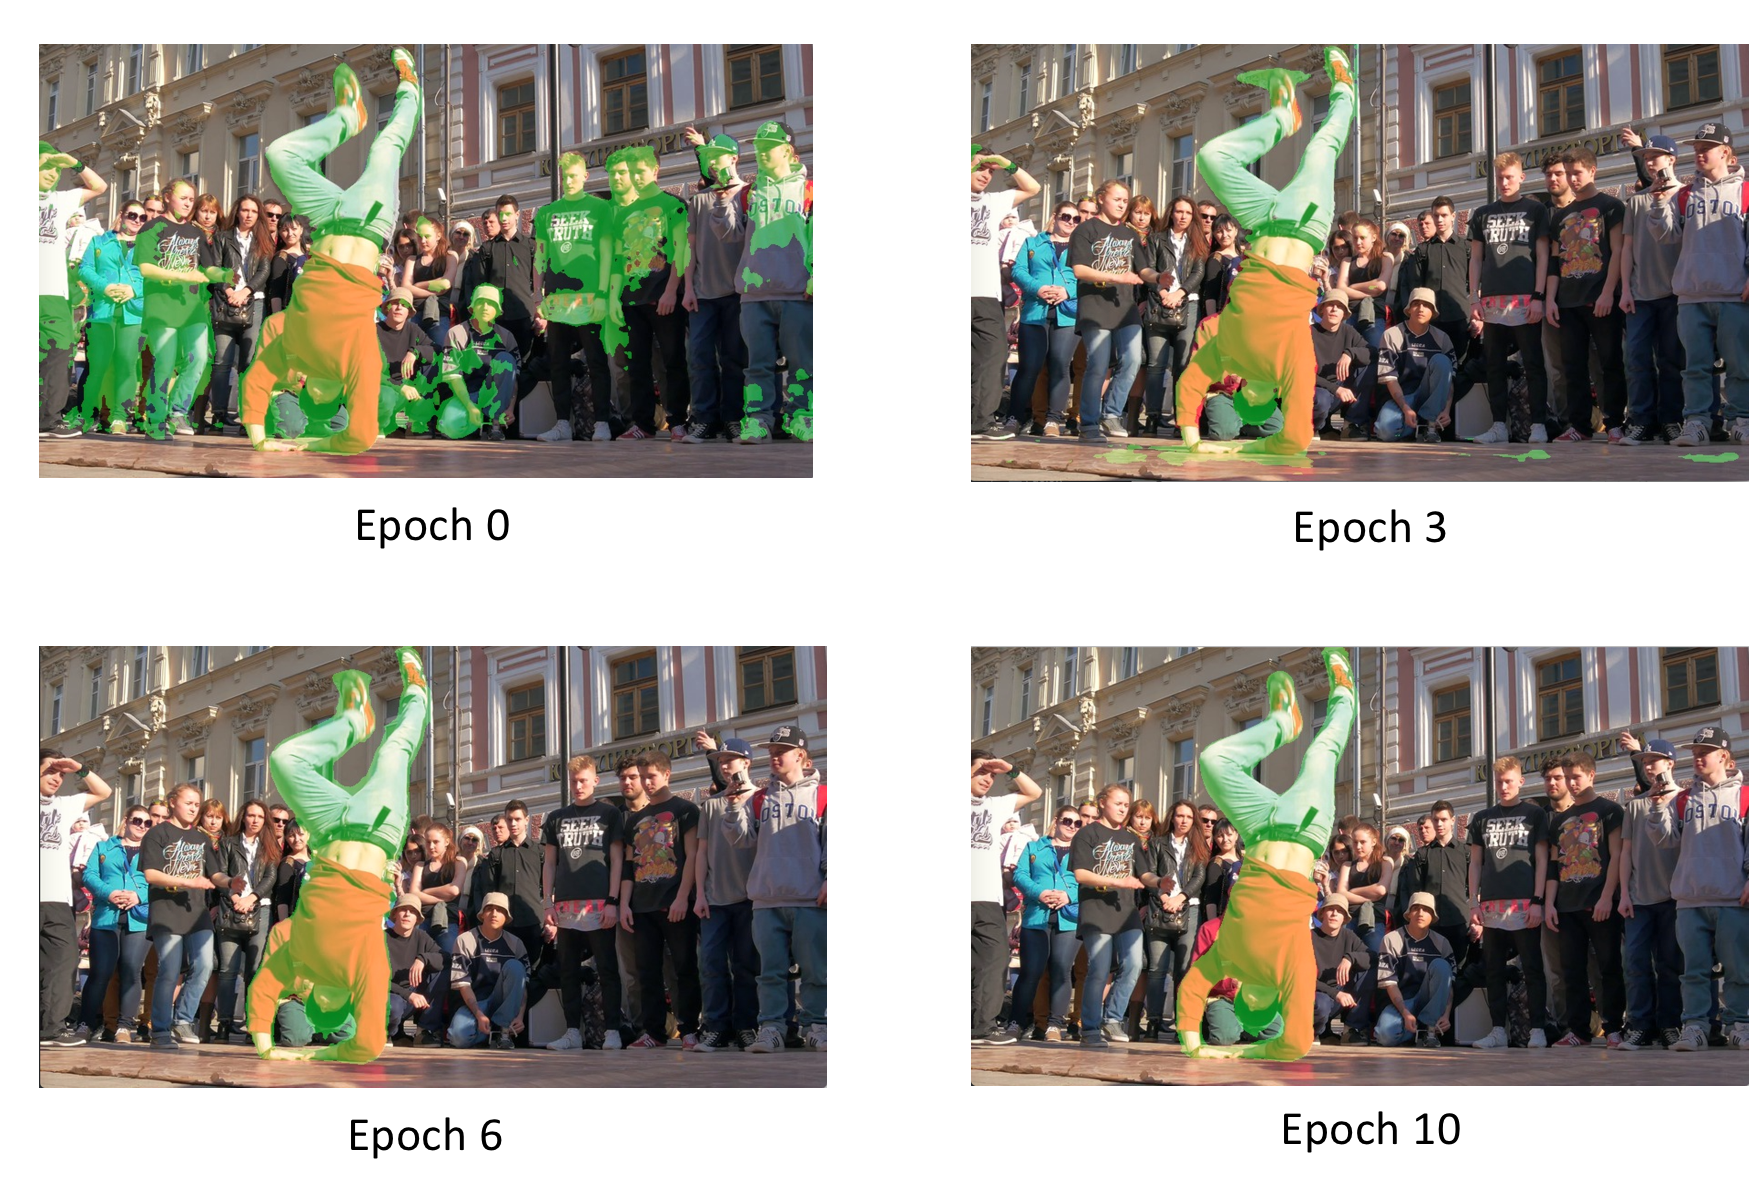
\includegraphics[width=0.8\textwidth]{./figure/fine_tune_result.png}
    \caption{Result of Fine-Tune with different train epoch}
    \label{fine_tune_result}
\end{figure*}


\subsubsection{Template Matching}
\textbf{Template Matching} based methods are widely used in visual tracking task\cite{OSVOS}\cite{OSVOS-S}\cite{BVS}\cite{PML}. Often, a fixed set of templates such as the masks of target objects in the first frame are used for matching targets. This paradigm fails in some challenging cases in DAVIS, as using a fixed set of templates cannot sufficiently cover large scale and pose variations. To mitigate the variations in both scale and pose across frames, exist-ing studies \cite{PML} exploit dynamic templates to maintain continuity of individual segmented regions across frames.

\textbf{OSVOS}\cite{OSVOS} based on a fully-convolutional neural network architecture that is able to successively transfer generic semantic information, learned on ImageNet\cite{Krizhevsky2012ImageNet}, to the task of foreground segmentation, and finally to learning the appearance of a single annotated object of the test sequence (hence one-shot). Although all frames are processed independently, the results are temporally coherent and stable. OSVOS processes each frame of a video independently(architecture has been shown in Fig.\ref{osvos_fcn}), obtaining temporal consistency as a by-product rather than as the result of an explicitly imposed, expensive constraint. 

In Fig.\ref{fine_tune_result}, we can find that accurate tracked object mask occurs along with the more train epochs, which means that the base network focus from general object to some specific tracked obeject.

\begin{figure}[ht]
    \centering
    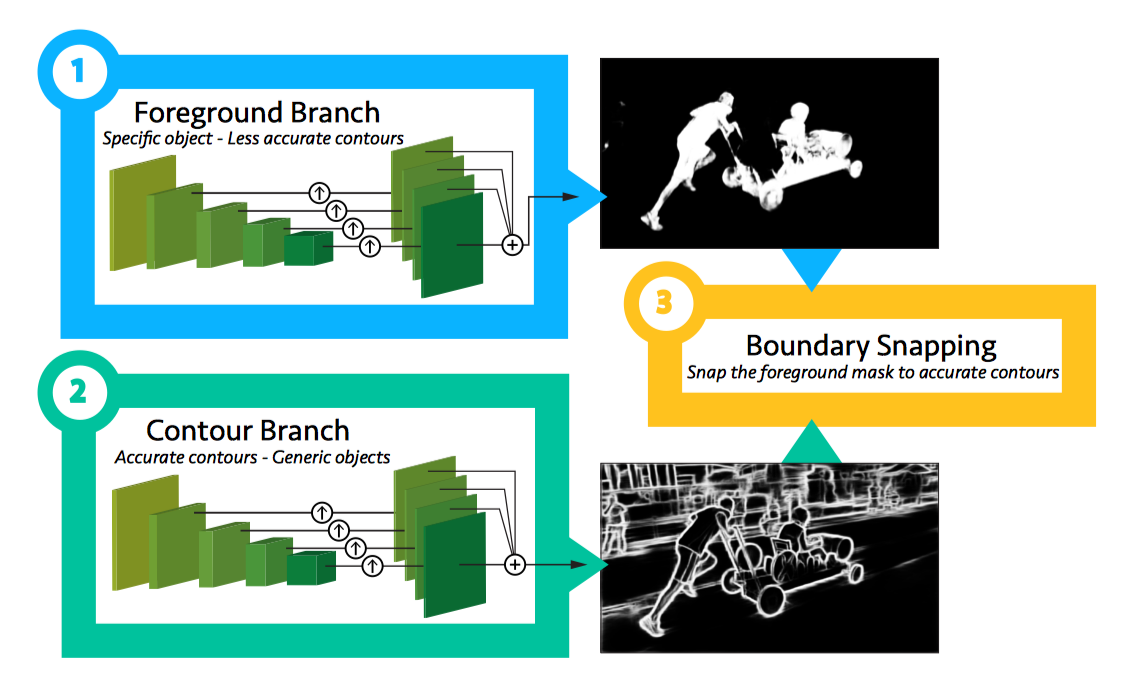
\includegraphics[width=0.5\textwidth]{./figure/osvos_fcn.png}
    \caption{VGG based two stream FCN}
    \label{osvos_fcn}
\end{figure}

OSVOS can work at various points of the trade-off between speed and accuracy. In this sense, it can be adapted in two ways. First, given one annotated frame, the user can choose the level of fine-tuning of OSVOS, giving him/her the freedom between a faster method or more accurate results. Experimentally, we show that OSVOS can run at 181 ms per frame and 71.5\% accuracy, and up to 79.7\% when processing each frame in 7.83 s. Second, the user can annotate more frames, those on which the current segmentation is less satisfying, upon which OSVOS will refine the result.

\begin{figure*}[ht]
    \centering
    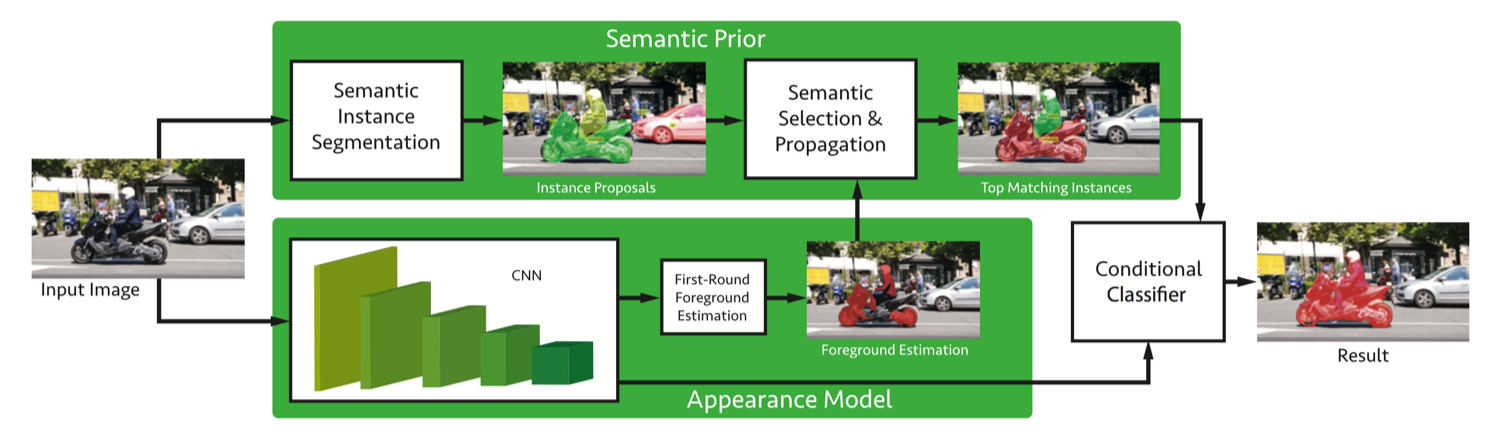
\includegraphics[width=\textwidth]{./figure/OSVOS_S.png}
    \caption{$\textbf{OSVOS}^\textbf{S}$ Network architecture overview: $\text{OSVOS}^\text{S}$ is composed of three major components: a base network as the feature extractor, and three classifiers built on top with shared features: a first-round foreground estimator to produce the semantic prior, and two conditional classifiers to model the appearance likelihood.}
    \label{OSVOS_S}
\end{figure*}


$\textbf{OSVOS}^\textbf{S}$\cite{OSVOS-S} based on a fully-convolutional neural network architecture that is able to successively transfer generic semantic information, learned on ImageNet, to the task of foreground segmentation, and finally to learning the appearance of a single annotated object of the test sequence (hence one shot). $\text{OSVOS}^\text{S}$ show that instance level semantic information, when combined effectively, can dramatically improve the results of previous method, OSVOS\cite{OSVOS}.

$\text{OSVOS}^\text{S}$ extends the model of the object with explicit semantic information. In the example of Fig.\ref{OSVOS_S}, for instance, $\text{OSVOS}^\text{S}$ would like to leverage the fact that segmenting an object of the category person and that there is a single instance of it. In particular, it will use an instanceaware semantic segmentation algorithm to extract a list of proposal of object masks in each frame, along with their categories. Given the first annotated frame, $\text{OSVOS}^\text{S}$ will infer the categories of the objects of interest by finding the best-overlapping masks.

$\text{OSVOS}^\text{S}$ can also work at various points of the trade-off between speed and accuracy, which is same with OSVOS. In this sense, given one annotated frame, the user can choose the level of fine-tuning performed on it, giving them the freedom between a faster method or more accurate results.


\textbf{BVS}\cite{BVS} propose a novel approach to video segmentation that operates in bilateral space, who design a new energy on the vertices of a regularly sampled spatiotemporal bilateral grid, which can be solved efficiently using a standard graph cut label assignment. Using a bilateral formulation, the energy that it minimize implicitly approximates long-range, spatio-temporal connections between pixels while still containing only a small number of variables and only local graph edges. 

\begin{figure}[ht]
    \centering
    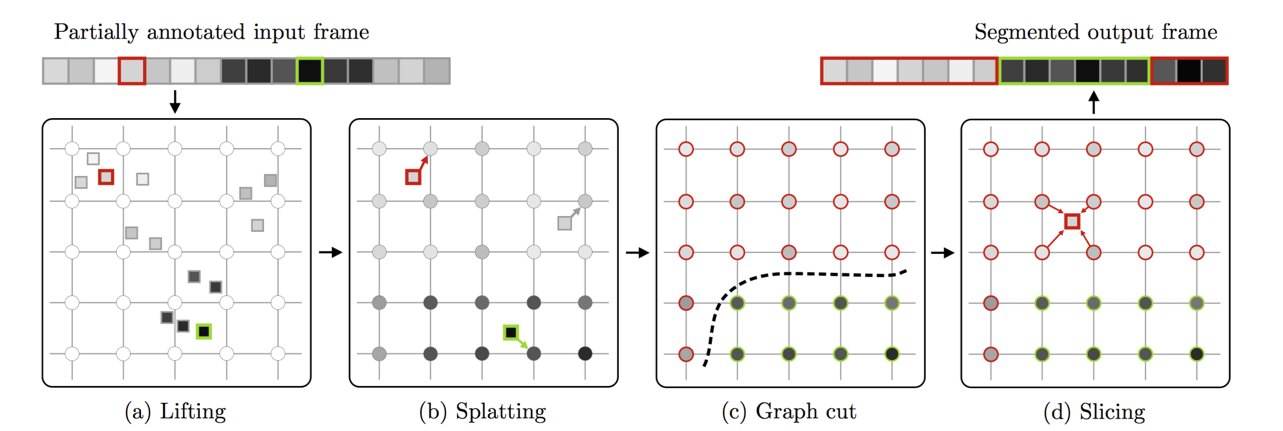
\includegraphics[width=0.5\textwidth]{./figure/BVS.png}
    \caption{\textbf{BVS} pipeline}
    \label{BVS}
\end{figure}

In Fig.\ref{BVS}, we show the pipline(demonstrated on a 1D example) of BVS: Pixels are lifted into a 2D feature space (a), with two user assigned labels (red and green highlighted pixels). Values are accumulated on the vertices of a regular grid (b), a graph cut label assignment is computed on these vertices (c), and finally pixel values are sliced at at their original locations (c), showing the final segmentation (again, red and green boundaries).


\textbf{PML}\cite{PML} embed pixels of the same object instance into the vicinity of each other, using a fully convolutional network trained by a modified triplet loss as the embedding model. Then the annotated pixels are set as reference and the rest of the pixels are classified using a nearest-neighbor approach. The proposed method supports different kinds of user input such as segmentation mask in the first frame (semi-supervised scenario), or a sparse set of clicked points (interactive scenario). details of PML is shown in Fig.\ref{PML}.

\begin{figure}[ht]
    \centering
    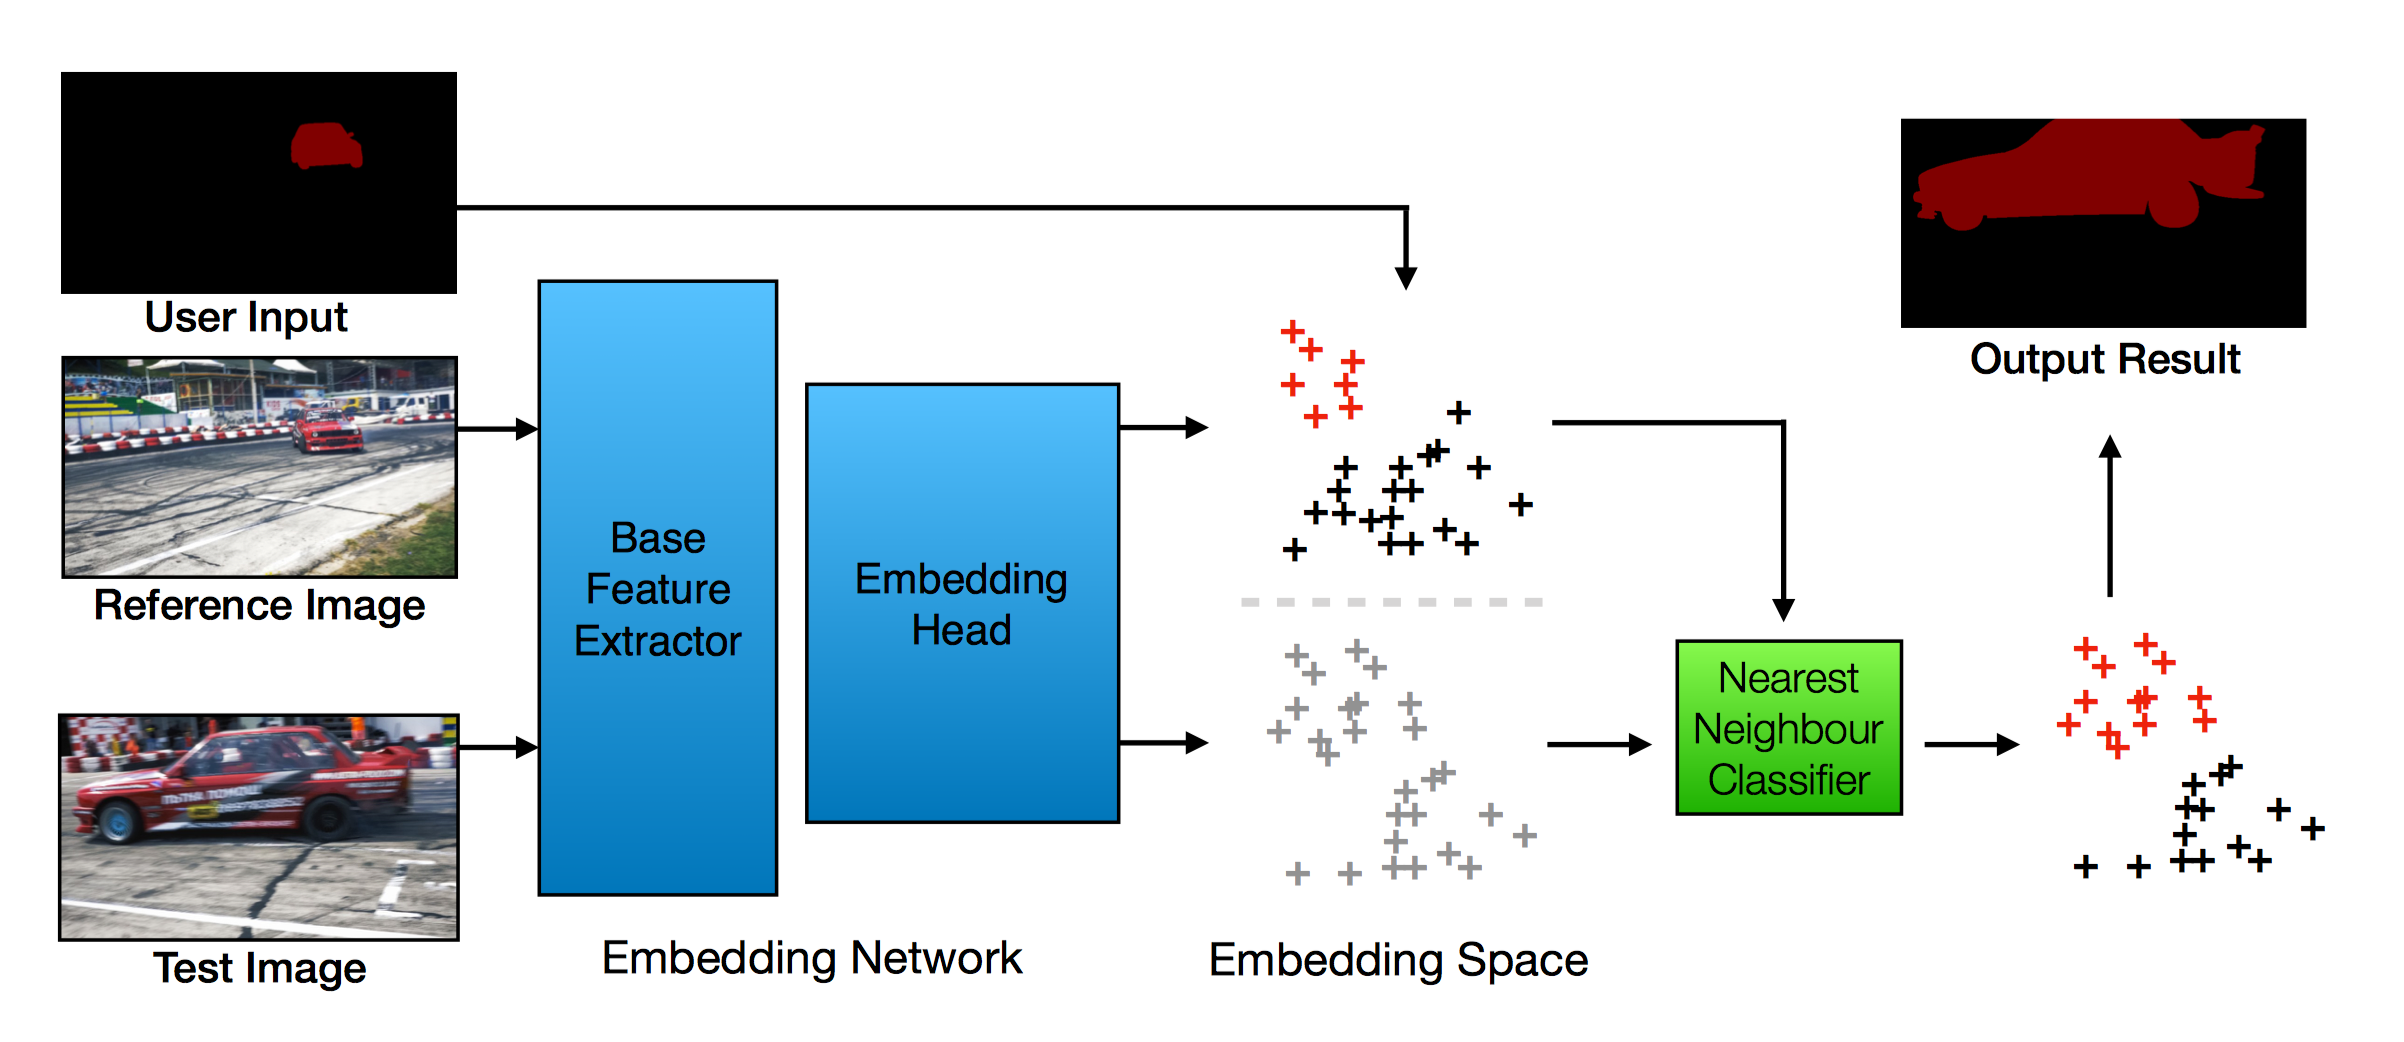
\includegraphics[width=0.5\textwidth]{./figure/PML.png}
    \caption{Overview of \textbf{PML}: Here we assume the user input is provided in the form of full segmentation mask for the reference frame, but interactions of other kind are supported as well}
    \label{PML}
\end{figure}

There are several main advantages of PML: Firstly, the proposed method is highly efficient as there is no fine-tuning in test time, and it only requires a single forward pass through the embedding network and a nearest-neighbor search to process each frame. Secondly, our method provides the flexibility to support different types of user input (i.e. clicked points, scribbles, segmentation masks, etc.) in an unified framework. Moreover, the embedding process is independent of user input, thus the embedding vectors do not need to be recomputed when the user input changes, which makes our method ideal for the interactive scenario.

\subsubsection{Temporal propagation}

\textbf{LucidTracker}\cite{LucidTracker} propose a new training strategy which is suitable for both single and multiple object tracking. Instead of using large training sets hoping to generalize across domains, it generate in-domain training data using the provided annotation on the first frame of each video to synthesize (``lucid dream'', which has been shown in Sec 2.4.2). This approach allows to reach competitive results even when training from only a single annotated frame, without ImageNet pre-training. LucidTracker indicate that using a larger training set is not automatically better, and that for the tracking task a smaller training set that is closer to the target domain is more effective. This changes the mindset regarding how many training samples and general ``objectness'' knowledge are required for the object tracking task.

\begin{figure}[ht]
    \centering
    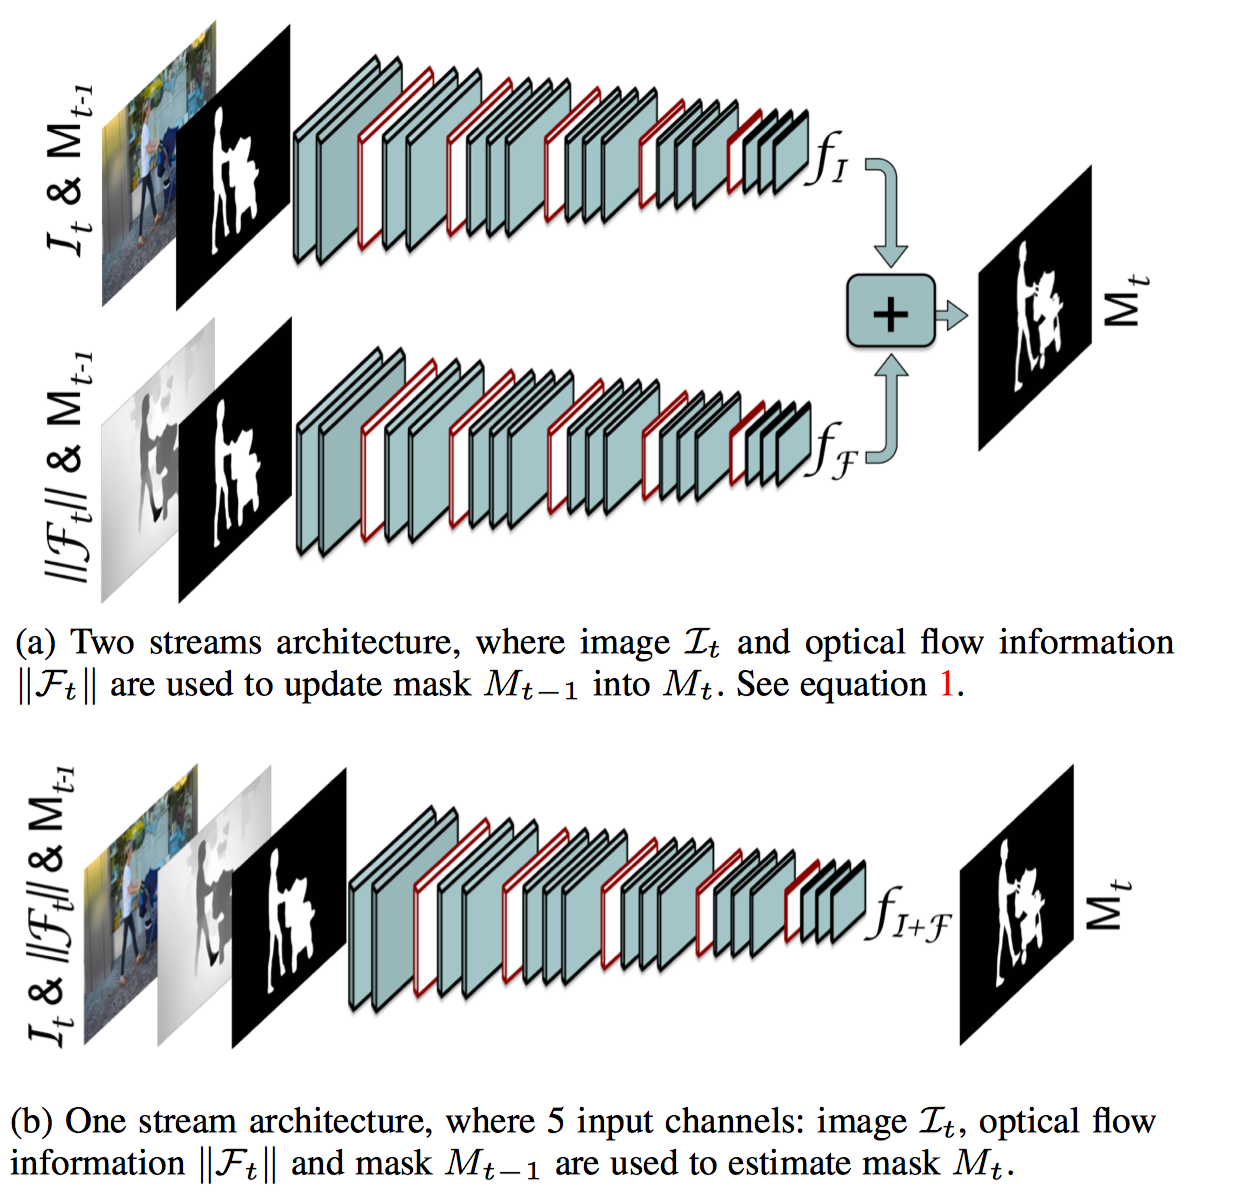
\includegraphics[width=0.5\textwidth]{./figure/lucid_tracker.png}
    \caption{Overview of the proposed one and two streams architectures in LucidTracker}
    \label{lucid_tracker}
\end{figure}

\begin{figure*}[ht]
    \centering
    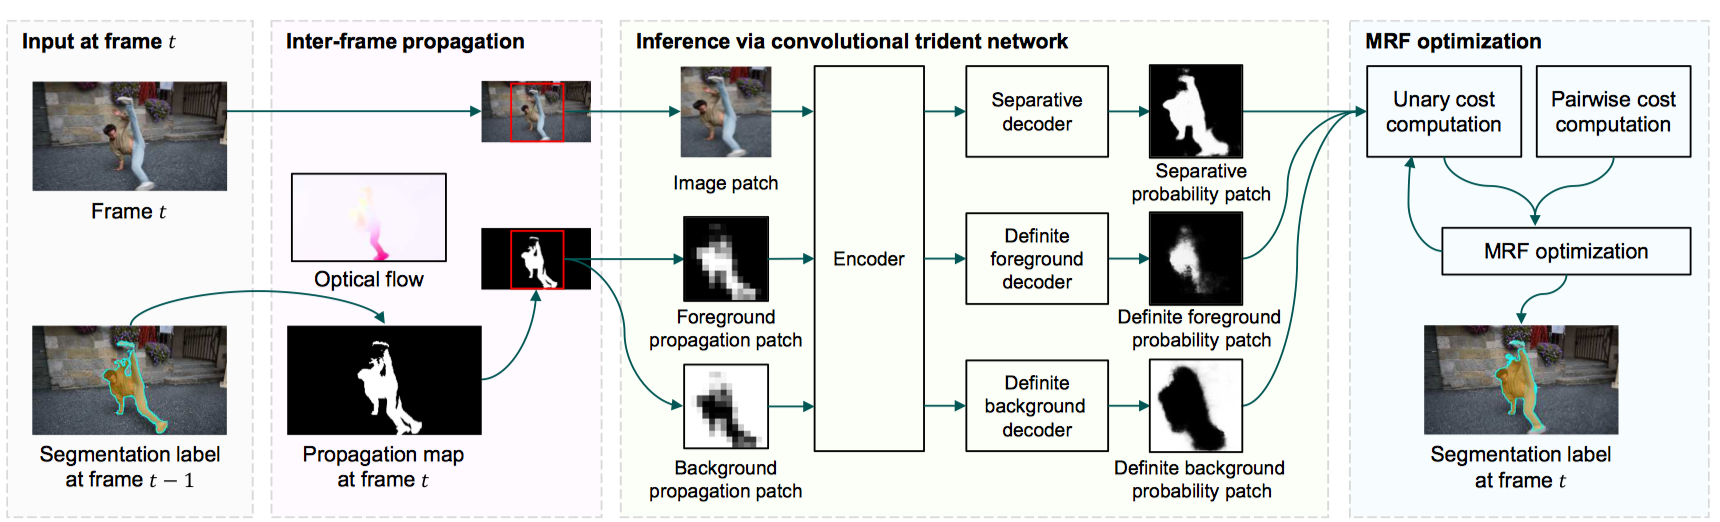
\includegraphics[width=\textwidth]{./figure/CTN.png}
    \caption{Overview of CTN}
    \label{CTN}
\end{figure*}

\textbf{CTN}\cite{CTN} propagate the segmentation labels at the previous frame to the current frame using optical flow vectors, has three decoding branches(Detail has been show in Fig.\ref{CTN}): separative, definite foreground, and definite background decoders. Then,CTN perform Markov random field optimization based on outputs of the three decoders. CTN sequentially carry out these processes from the second to the last frames to extract a segment track of the target object. 

\textbf{MaskRNN}\cite{MaskRNN}


\subsubsection{Combine}

\textbf{OSMN}\cite{OSMN}

\textbf{DyeNet}\cite{DyeNet} formulate a deep recurrent network that is capable of segmenting and tracking objects in video simultaneously by their temporal continuity, yet able to re-identify them when they re-appear after a prolonged occlusion. DyeNet combine both temporal propagation and re-identification functionalities into a single framework that can be trained end-to-end. In particular,it present a re-identification module with template expansion to retrieve missing objects despite their large appearance changes. In addition, it contribute a new attention-based recurrent mask propagation approach that is robust to distractors not belonging to the target segment.

\begin{figure*}[ht]
    \centering
    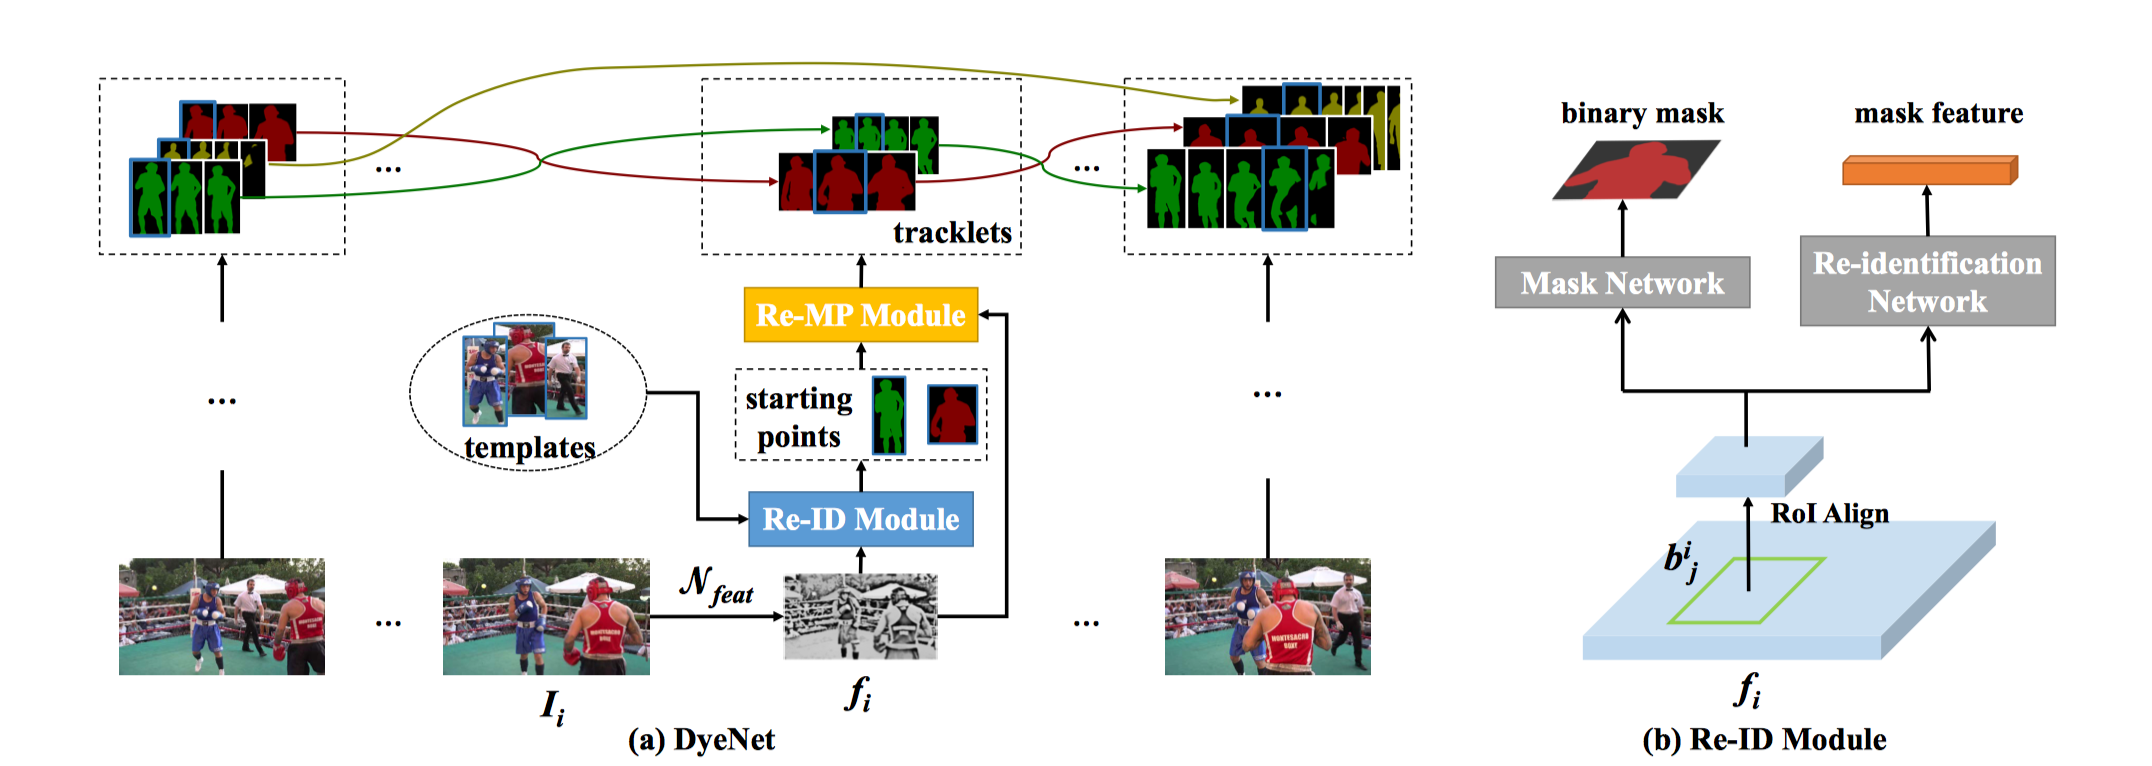
\includegraphics[width=\textwidth]{./figure/DyeNet.png}
    \caption{(a) The pipeline of \textbf{DyeNet}. The network hinges on two main modules, namely a re-identification (Re-ID) module and a recurrent mask propagation (Re-MP) module. (b) The network architecture of the re-identification (Re-ID) module.}
    \label{DyeNet}
\end{figure*}

DyeNet joints template matching and temporal propagation into a unified deep neural network for addressing video object segmentation with multiple instances(detail is shown in Fig.\ref{DyeNet}). The network can be trained end-to-end. It does not require online training (i.e., fine-tune using the masks of the first frame) to do well but can achieve better results with online training.In addition, DyeNet present an effective template expansion approach to better retrieve missing targets that reappear with different poses and scales.




\subsection{Unsupervised VOS}
Video object segmentation is the task of extracting spatio-temporal regions that correspond to object moving in at
least one frame in the video sequence. In contrast to semi-supervised VOS, unsupervised video object segmentation have 
more challages and is more practical in real world. In real world case, with the limitation of resources and the diversity of scenario,
it is difficult to simulate various outdoor scenario and collect dataset from it in laboratory. So unsupervised video object 
segmentation have more important impact on our real daily life. To better understand to unsupervised setting, here we list some
obvious difference between semi-supervised video segmentation.
\begin{enumerate}
    \item no first frame groundtruth is provided in test phase.
    \item no finetune process in test phase is needed.
\end{enumerate}

In unsupervised VOS tasks, we can regard them as zero-shot video objects segmentation. Because we cannot have any objects priors
in test phase, namely that the objects in testset does not exit in training phase. The task's main challages is that we need to infer
the primary objects which are moving in video frames automatically. The algorithm can discovers the most salient, or primary, objects,
that move against a video's background or display different color statistics. To better capture the moving objects against the background,
the object motion is the critical cue for identify salients objects throught entire video sequences. Next, we will introduce some important
methods which is commonly used in unsupervised VOS.

\begin{figure*}
    \begin{center}
    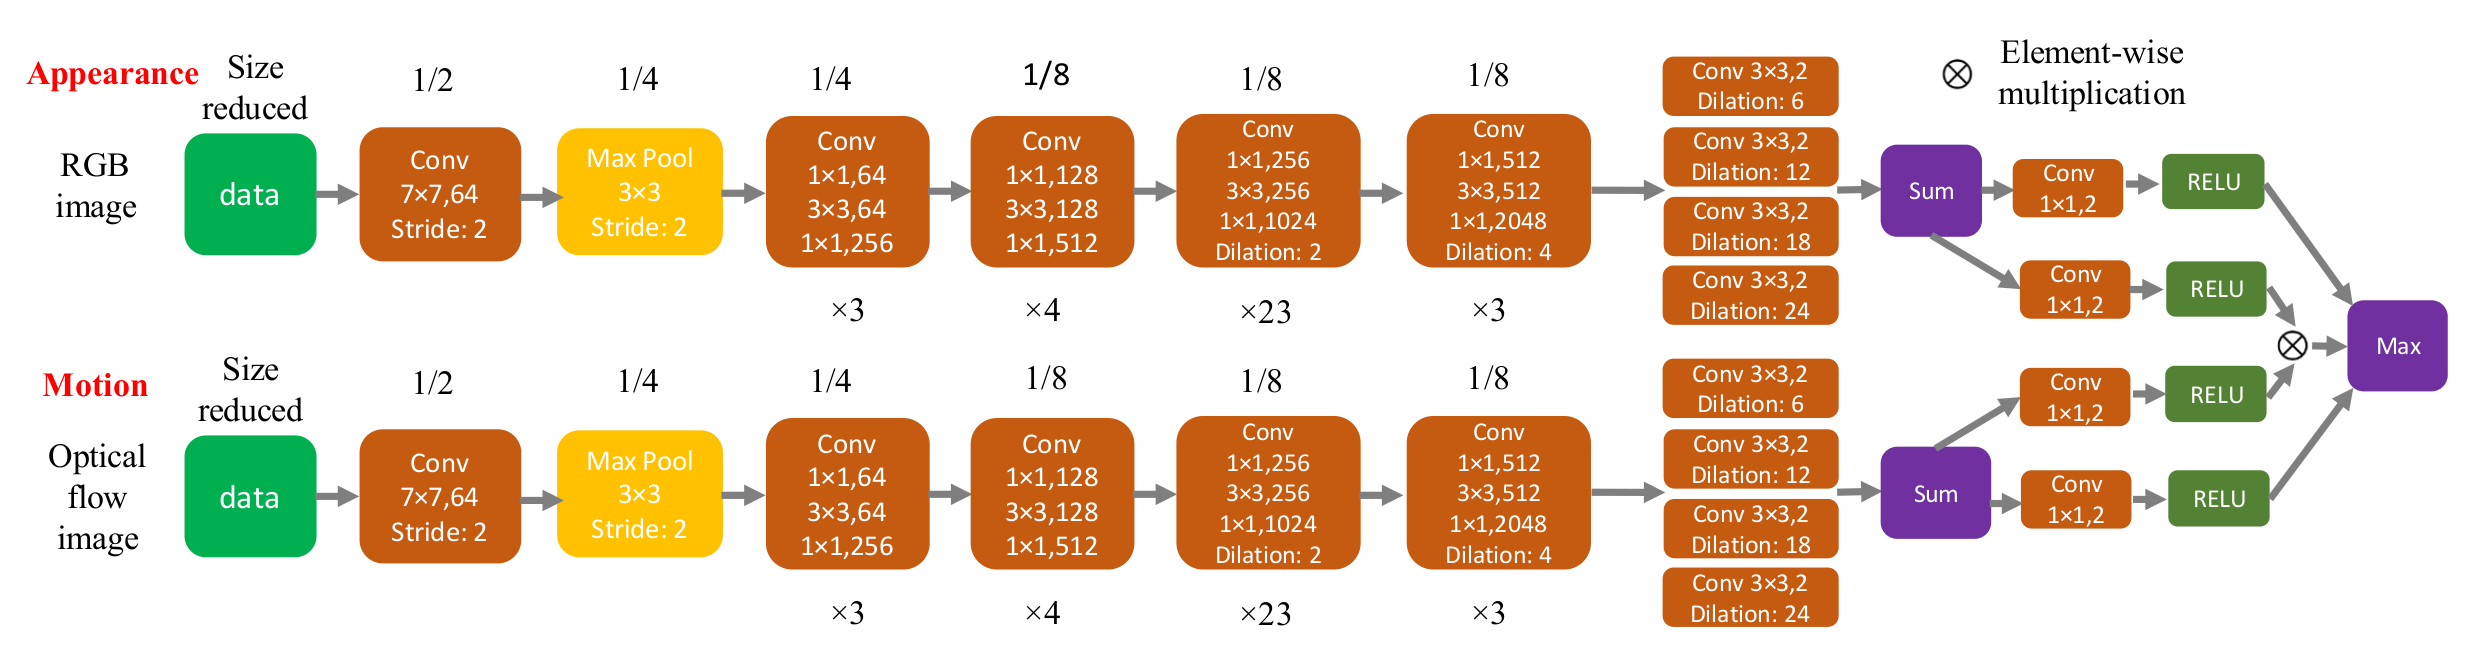
\includegraphics[width=\textwidth]{figure/FSEG_NET.png}
    \end{center}
    \caption{FSEG Network}
    \label{FSEG}
\end{figure*}

\subsubsection{Motion in Video Sequences}
In traditional static image semantic segmentation, the apperance information play an import role, which means that 
the performance is enough good if we can extract more reliable apperance features. But in video setting, thera are various
difficult challlenges caused by object moving, which are motion blur and ambigious and occluated. We just rely on apperance information
, which can  fail in this specifical scenario. Motion information can greatly help reduce this ambigious. We can capture more temporal information
to help locate objects in videos frames.

Jain $et.al$ \cite{Jain2017FusionSeg} propose an end-to-end learning framework for segmenting generic objects in video,
which learns to combine appearance and motion information to produce pixel level segmentation masks for all prominent objects.
They design a two-stream fully convolutional neural network which fuses together motion and apperance in a unified framework.

As shown in Fig \ref{FSEG}, the network can take two different inputs, which are raw images and optical flow images respectively.
The motion branch can map the motion into foreground objects, which can greatly capture temporal infomation.
In the last fusion stage, this method does not simply concat two stream feature to get the final prediction.
They design a new fusion strategy to create three independent parallel branches. They apply $1\times1$ convolution to apperance and
motion branch. Finally they apply a layer that thkes the elements-wise maximum to obtain the final prediction. The movivation is that 
an object segmentation prediction is reliable if 1) either apperance or motion model along predicts the object 
segmentation with very strong confidence or 2) their combination together predicts the segmentation with high confidence. 

Besides the two stream strategy, there are still the other fusion strategy to fuse the motion information into apperance 
features to provide additional infomation for building a strong representation of objects that evolves over time. 

\begin{figure}[ht]
    \centering
    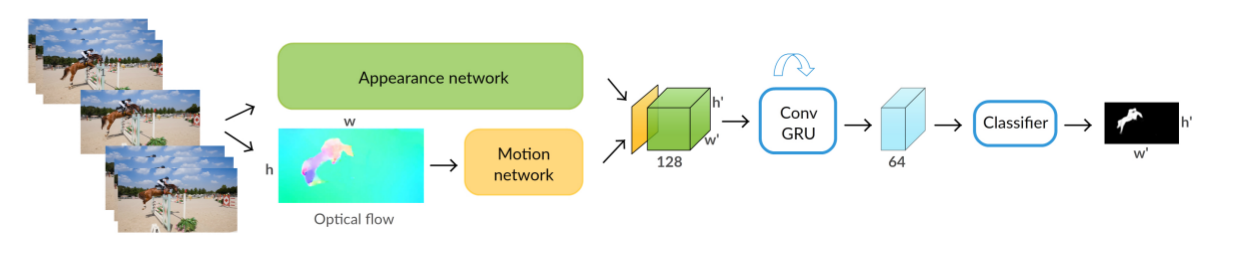
\includegraphics[width=0.5\textwidth]{./figure/LVO_NET.png}
    \caption{LVO Network}
    \label{LVO}
\end{figure}

Pavel $et.al$\cite{Tokmakov2017Learning} proposed a new network structures. In Fig\ref{LVO}, they use a motion network to extract motion features, which 
take as side information to get the final prediction. The motion network is a pretrained network.

We can improve the performance by combining apperance feature and motion features. However, how can we get good motion
prediction by inputing optical flow images. Pavel $et.al$\cite{LMPV} proposed a encoder-decoder style to estimate the motion 
of video directly.

\begin{figure}[ht]
    \centering
    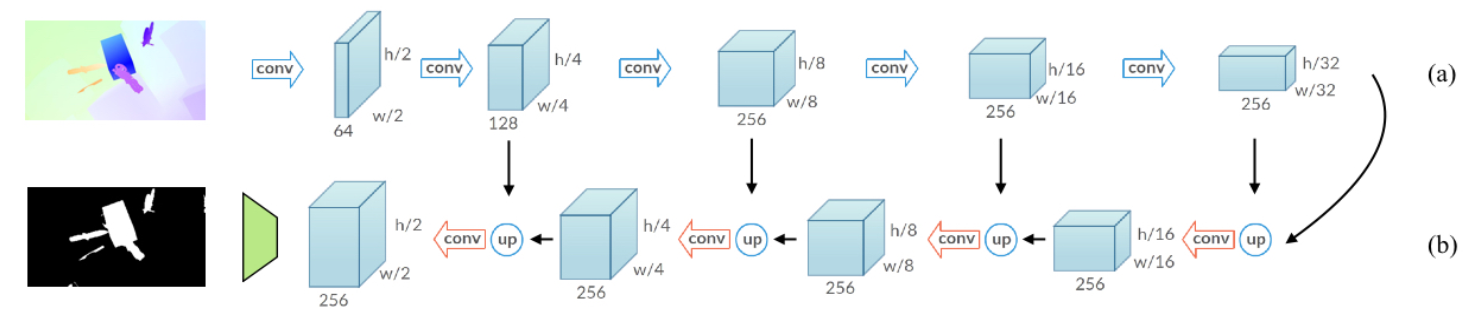
\includegraphics[width=0.5\textwidth]{./figure/LMP_NET.png}
    \caption{LMP Network}
    \label{LMP}
\end{figure}

In Fig.\ref{LMP}, the input is the optical flow and the output is the moving probability of every single pixel. They use the U-net structure, which
add some shortcut connection to add the coarse information to high level feature, which will greatly help enhance the feature representation power.
After getting the motion map, we can directly use this to predict foreground objects in frames. 

\begin{figure}[ht]
    \centering
    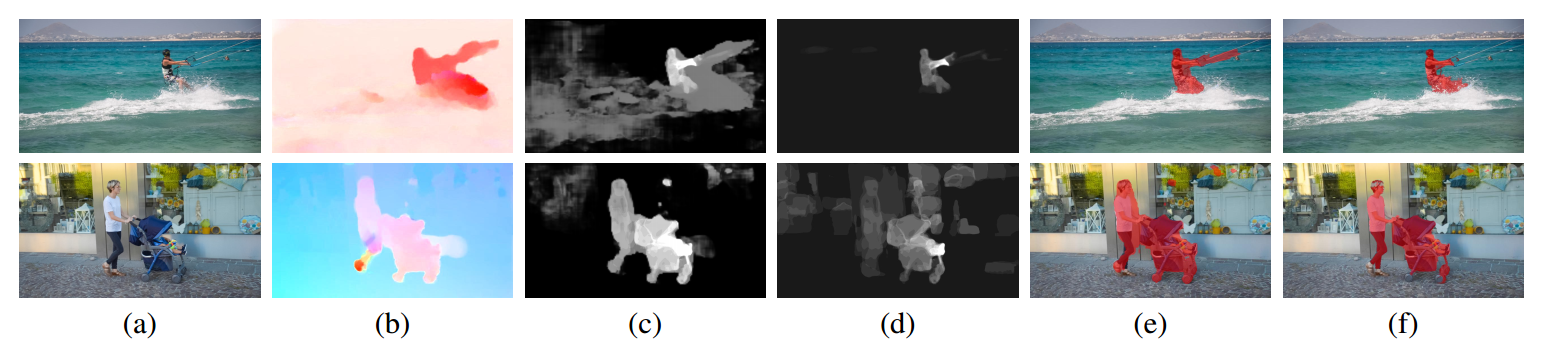
\includegraphics[width=0.5\textwidth]{./figure/LMP_results.png}
    \caption{LMP Segmentation Pipeline}
    \label{LMP_results}
\end{figure}

Fig.\ref{LMP_results} is the whole pipeline using motion map to predict the final foreground objects. Each row shows: (a) raw images,
(b) optical flow estimated with LDOF \cite{brox2009large}, (c) output of motion network with LDOF flow as input, (d) objectness map computed with
proposals \cite{pinheiro2016learning}, (e) initial moving object segmentation result, (f) refined result with CRF.

We can observe that mapping motion prediction to final foreground segmentation is a realiable methods. The temporal cue can provide more realiable
feature to help do prediciton. So it is critical to advantage the motion cue.


\subsubsection{Visual Memory in Video Sequences}
Motion cue can greatly help capture temporal information. However, motion just can capture the substantial frames and cannot encode more long range
temporal information over several frames. In reality, the RNN have nature attributes that encoder long time dependency. However, the RNN just can 
receive the vector. So representation power is very limited. So Pavel $et.al$\cite{Tokmakov2017Learning} replace the vector in LSTM by the convolution 
operation, which can greatly improve representation power and is more suitable for video segmentation task.
\begin{figure}[ht]
    \centering
    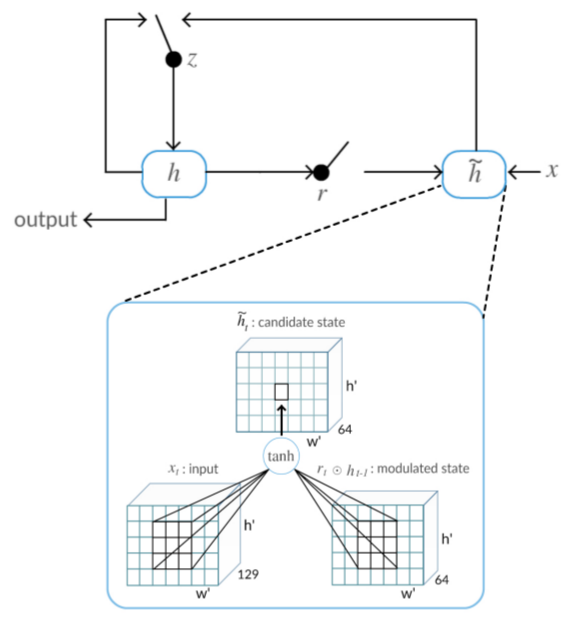
\includegraphics[width=0.35\textwidth]{figure/LVO_CONVRRU.png}
    \caption{convolutional GRU}
    \label{CONVGRU}
\end{figure}

\begin{align}
     z_t &= \sigma(x_t*w_{xz} + h_{t-1}*w_{hz}+b_z) \\
     r_t &= \sigma(x_t*w_{xr} + h_{t-1}*w_{hr}+b_r) \\
     \hat{h}_t &= tanh(x_t*w_{x\hat{h}} + r_t \odot w_{h\hat{h}}+b_{\hat{h}}) \\
     h_t &= (1-z_t) \odot h_{t-1} + z_t \odot \hat{h}_t
\end{align}

Here is the update equation in CONVGRU, where the $*$ is the convolution operation and $\odot$ denote the elements-wise product.
We can see from Fig.\ref{CONVGRU} that they replace the linear combination by convolution operations and a tanh nonlinearity. For frame $t$ in the video
sequence, ConvGRU uses the two stream representation $x_t$ and previous state $h_{t-1}$ to compute the new state $h_t$. The dynamics of this computaiton 
are guided by an update gate $z_t$, a forget gate $r_t$, The states  and the gates are $3$D tensor, and can cahracterizer spatio-temporal pattern in
the video, effectively memorizing which objects move and where they move to. The ConvGRU applies a total of six convolutional opeartions at each time step.
All operation are fully differentiable. So the parameters of the convolution can be trained in an end-to-end fashion wiht back propagation through times.
But there are some drawbacks that the network is memory-comsuming. It's very hard to train. 
\begin{figure}[ht]
    \centering
    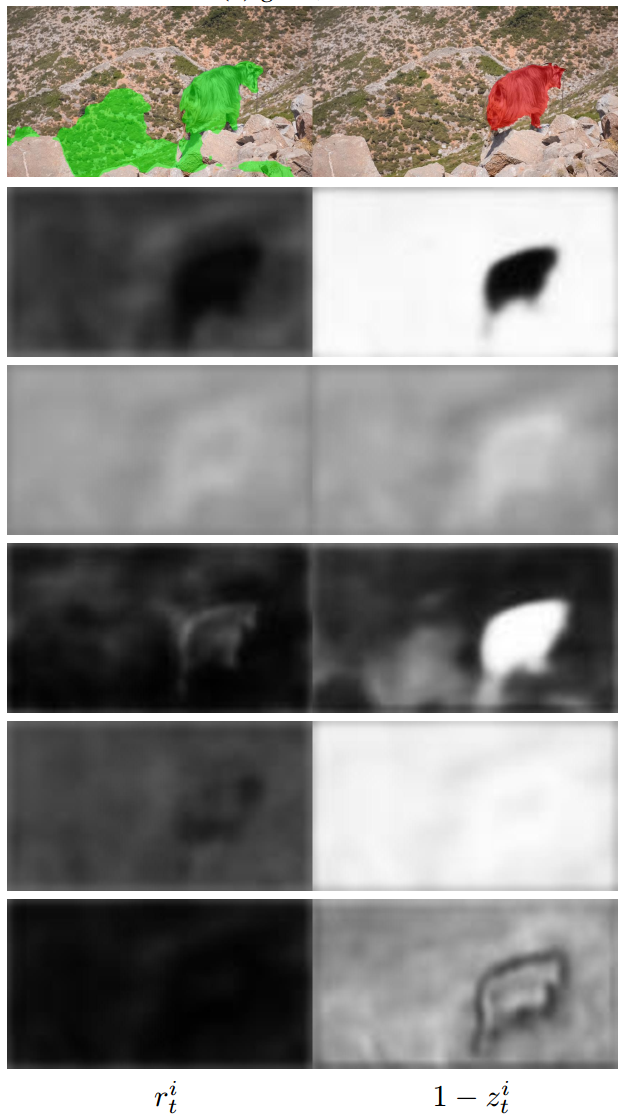
\includegraphics[width=0.35\textwidth]{figure/visual_memory.png}
    \caption{Visual memory in ConvGRU}
    \label{vis}
\end{figure}

We can see the from Figure \ref{vis}, The outputs of the motion stream alone (left) and the final segmentation result (right) of the two examples are
shown in the top row in the figure. The five rows below correspond each to one of the 64 dimensions of $r_t$ and $(1− z_t)$.
These activations are shown as a grayscale heat map. 
High values for either of the two activations increases the influence of the previous state of a ConvGRU unit in the computation of the new state matrix. 
If both values are low, the state in the corresponding locations is rewritten with a new value. 
For the second row in Figure \ref{vis}, we observe the update gate being selective based on the appearance information, i.e., it updates the
state for foreground objects and duplicates it for the background. Note that motion does not play a role in this case.
This can be seen in the example of stationary people (in the
background) on the right, that are treated as foreground by
the update gate.

In the paper, the author proposed a bidirectional CONVGRU, which can encode motion from the fisrt frame and the last from. This technicial can improve the feature
representation power further. As the expriments shown, the bidirectional CONVGRU bring $5\%$ improvements.

\subsubsection{Hand Craft Methods}

As we all know, deep learning method make huge progress in computer vision. Howerver, there are still a mount of traditional method based on 
hand craft features, which can produce comparable result with deep learning. Sometimes the traditional method is easy to explainable and stable.

Most current methods for unconstrined fg/bg video segmentation are graph-based \cite{Lee2011Key, Papazoglou2013Fast, zhang2013video}. The video
is represented using an Markov Random Field graphical model which consist of a fg/bg data term for each pixel and pairwise
terms between neighboring pixels. The data term is iteratively refined by learning learning color model of the foreground
and background. For computational reasons, the pairwise  terms are typical considered only between adjacent pixels inthe same 
frame and corresponding pixels in adjacent frames(using optical flow).

